We conducted a review of literature with search query including the words \textit{security}, and \textit{hackathon} to select papers relevant to security hackathons. This resulted in 440 results which were closely analysed to remove results that did not apply leaving 22 papers.

\begin{table*}[h]
    \centering
    \caption{Hackathons in security}
    \label{tab:hackinsecurity}
    \begin{tabular}{|p{0.3\linewidth}|p{0.3\linewidth}|p{0.3\linewidth}|} \hline
        Research & Makeathon & Gamification \\ \hline
\cite{kharchenko2016university}, \cite{foley2018science}, \cite{key2017automotive}, \cite{lin2019using} & \cite{kharchenko2016university} \cite{dainotti2018bgp}, \cite{melon2018eve}, \cite{starov2015hacking}, \cite{sherman2019cats}, \cite{weiss2015teaching}, \cite{abdullah2015stimulating}, \cite{balcerzak2017press}, \cite{uys2019hackathons} & \cite{sherman2019cats},\cite{boopathi2015learning}, \cite{flood2012black}, \cite{vykopal2017lessons}, \cite{ricci2016cybersecurity}, \cite{davis2014fun}, \cite{lorenz2019cybersecurity}, \cite{katsantonis2017conceptual}, \cite{coull2017gamification}, \cite{dupuisevaluating}\\ \hline
    \end{tabular}
\end{table*}

\begin{figure}[h]
%\vspace{-15pt}
  \centering
  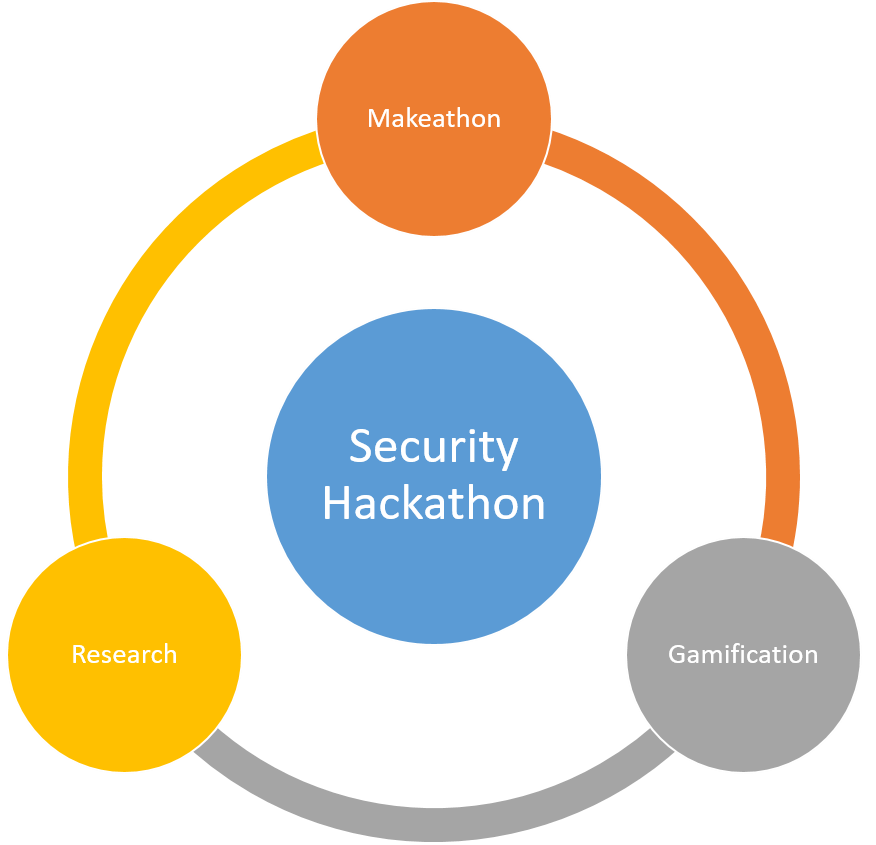
\includegraphics[width=0.75\linewidth]{Hackcycle.png}
  \caption{Hackathons in Security} \label{Fig:hackcycle} 
 % \vspace{-20pt}
\end{figure}

\subsection{Related work}

Related works exist where perceived learning in security hackathons is mentioned or discussed. 

[\textit{...add more related works}]

Finally, research by \cite{foley2018science}, briefly mentions learning within collaboration with other participants with expertise in cybersecurity. 

However, there are not yet studies evaluating perceived learning and the activities to influencing learning in security hackathons.


Learning according to the Merriam-Webster dictionary\footnote{https://www.merriam-webster.com/dictionary/learning}, is the "activity or process of gaining knowledge or skill by studying, practicing, being taught, or experiencing something". Research has shown that learners employ different approaches to learning based on perceptions of the learning environments \cite{entwistle1991approaches,marton1997approaches}. % based on the learners' perceptions of the learning environment .% -- surface, relating ideas and deep approaches.

\begin{comment}
\textbf{WINNER - Alfred}: Pipedrive for CSOs. Alfred shows you where you are, where you need to go and what exactly you need to do next to achieve the security program health you deserve. \newline
\textbf{Prize}: Straight pass to Ajujaht TOP 100\footnote{https://www.ajujaht.ee/event/ajujahi-top-100-pitch/}; Latitude59\footnote{https://latitude59.ee/} tickets; access to Startup Wise Guys\footnote{\label{SWPfoot}https://startupwiseguys.com/} online cybersecurity pre-acceleration program.

\textbf{1st Runner-Up - SecureMVP:}
SecureMVP sought to help startups to be more security-aware right from its ideation phase in order to produce a secure minimum viable product (MVP). The solution provides security status report with risks and a to-do lists to enhance security. \newline
\textbf{Prize}: sTARTUp Day tickets and access to Startup Wise Guys\footnoteref{SWPfoot} online cybersecurity pre-acceleration program.

\textbf{2nd Runner-Up - Chatrino:} Chatrino provides an innovative way to securely and untraceably send messages over the internet.\newline
\textbf{Prize}: Access to Startup Wise Guys\footnoteref{SWPfoot} online cybersecurity pre-acceleration program; business lunch with a possible security investor %F-secure.
\end{comment}

\begin{comment}
The post-hackathon phase will cover specific points such as project continuation, community building, career paths and learning paths developed. 
\end{comment}

% In the pre-hackathon/idea garage event survey, we ascertained participants' basic demographics, baseline competence in security, learning expectations for the hackathon, and intentions to attend the coming hackathon. We also asked about the security idea generation and the satisfaction with the pre-hackathon event. In the post-hackathon survey, we measured the respondents attitude towards the hackathon, and their perceived learning experience, derived from our interventions. 

\begin{comment}
\begin{table*}[h]
    \centering
    \caption{Skill demographics of registered participants}
    \label{tab:skilldemo}
    \begin{tabular}{|p{0.2\linewidth}|p{0.2\linewidth}|p{0.2\linewidth}|p{0.2\linewidth}|} \hline
    Participant category & Security-oriented & software development oriented & product oriented participants \\ \hline
    Total & 9 & 71 & 18\\ \hline
        \end{tabular}
\end{table*}
\end{comment}

 %where each participant could form a team with other participants based on common interest in an idea. 
%Since hackathons run on collaboration basis, the process of team formation is centered . %Opportunities were provided for team formation including; (1) mentor suggestion of the mix of skills required for the proposed project, (2) opportunity for networking for familiarisation before forming a team at hackathon pre-event, (3) exercise that allows any participant to sign on for roles in teams of interest.

\begin{table}[h]
    \begin{tabular}{|p{0.2\linewidth}|p{0.2\linewidth}|p{0.2\linewidth}|p{0.2\linewidth}|}
    \hline
   \multicolumn{4}{|c|}{1. \textbf{Observation of students use of Intervention}}\\ \hline
    \textbf{Intervention} & Beginning & Midway & End \\ \hline
    Idea generation & & & \\ \hline
    Security Talks & & & \\ \hline
    Mentor Feedback & & & \\ \hline
    Competition based & & & \\ \hline
    \multicolumn{4}{|c|}{2. \textbf{Interest in the topic }}\\ \hline
     \multicolumn{4}{|c|}{} \\ \hline
     \multicolumn{4}{|c|}{3. \textbf{Attitude to mentors }}\\ \hline
     \multicolumn{4}{|c|}{} \\ \hline
     \multicolumn{4}{|c|}{4. \textbf{Assessment of participant satisfaction }}\\ \hline
     \multicolumn{4}{|c|}{} \\ \hline
    \end{tabular}
    \caption{Observation Scheme}
    \label{tab:observescheme}
\end{table}

%By observation, the idea generation sessions were appreciated and enabled participants to freely speak about their ideas. Although some ideas were reported to have been generated at the spot, there were also ideas that have been previously evaluated at the pre-hackathon event or at participants workplace.  Security talks were an interesting part for the participants....

%Observation scheme is measured by these five marks: 5-stable, 4- constant, 3 - persistent, 2 - diffused, 1 - absent. 


\begin{comment}
\subsubsection{cybersecurity expertise}
Since this is a cognitive process, the measure of security knowledge possessed by the participants was asked. There was a comparable cybersecurity expertise ($Mdn =3, IQR = 1$). However, most respondents were new to security-focused hackathon events, accounting for 84.6\% of the respondents and did not participate in any preparatory actions for the hackathon ($Mdn = 1$) such as developing a security related project idea or learning about topics that would be useful for the security project.

\begin{figure}[h]
%\vspace{-15pt}
  \centering
  \includegraphics[width=\linewidth]{cybersecexp.JPG}
  \caption{Self-estimation of cybersecurity experience} \label{Fig:cyberexp} 
 % \vspace{-20pt}
\end{figure}
\end{comment}
\begin{table*}[h]
    \centering
     \begin{tabular}{|p{0.22\linewidth}|p{0.13\linewidth}|p{0.13\linewidth}|p{0.13\linewidth}|p{0.13\linewidth}|p{0.13\linewidth}|p{0.13\linewidth}|}
    \hline
      & \multicolumn{6}{c|}{The cognitive process dimension}  \\ \hline
	The knowledge dimension & Remember & Understand  & Apply & Analyse & Evaluate & Create \\ \hline
	Factual Knowledge & List & Summarize & Classify & Order & Rank & Combine \\ \hline
	Conceptual & Describe & Interpret & Experiment & Explain & Assess & Plan \\ \hline
	Procedural & Tabulate & Predict & Calculate & Differentiate & Conclude & Compose \\ \hline
	Meta-cognitive & Appropriate use & Execute & Construct & Achieve & Action & Actualise \\ \hline
    \end{tabular}
    \caption{Blooms Taxonomy categories}
    \label{tab:bloomsubcategories}
\end{table*}

\begin{table}[h]
    \centering
    \caption{Findings of result of survey}
    \label{tab:Surveydata}
    \begin{tabular}{|p{0.2\linewidth}|p{0.2\linewidth}|p{0.2\linewidth}|p{0.2\linewidth}|} \hline
    Participant category & Security-oriented & software development oriented & product oriented participants \\ \hline
    Total & 9 & 71 & 18\\ \hline
        \end{tabular}
\end{table}

Team 1 showed an understanding of the cybersecurity theme of the hackathon and was able to describe their solution by highlighting the security issue to be addressed, how the solution addresses this issue and why this security issue is important to be fixed.

Team 1 was able to interpret this security solution into a tool/process.


Learning Objectives

\begin{enumerate}
    \item Remember and understand security concepts presented through the introduced interventions.
    \item Use the security knowledge gained into developing an idea that solves current security issues.
    \item Develop and present a viable prototype that demonstrates the outcome of acquiring security knowledge and using it to solve security issues.
    %\item Present the developed solution and its security 
\end{enumerate}


\begin{comment}

\begin{figure}[h]
%\vspace{-15pt}
  \centering
  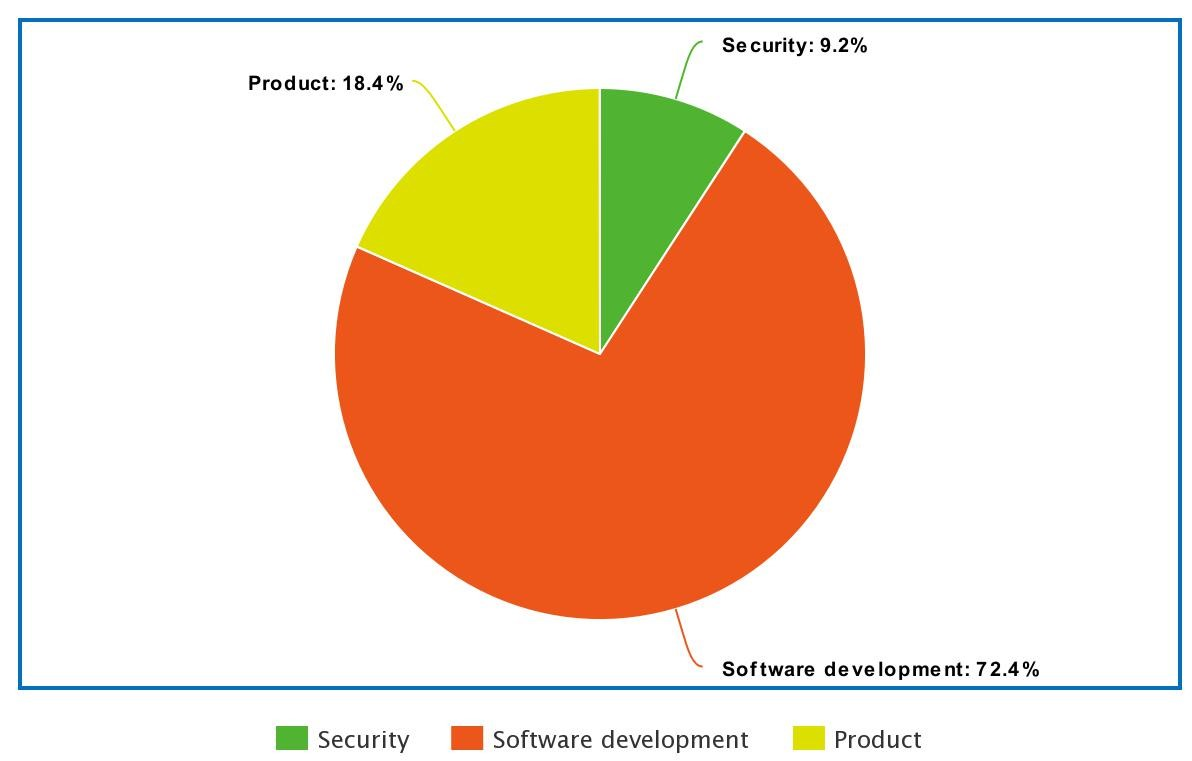
\includegraphics[width=\linewidth]{skilldemographics.jpeg}
  \caption{Skill demographics of registered participants} \label{Fig:skilldemo} 
 % \vspace{-20pt}
\end{figure}
\end{comment}

These data sources are used to discuss answers to the following questions;
\begin{enumerate}
    \item Which interventions were the most useful in influencing higher level of cybersecurity in Team B as analysed in Section \ref{teamcomparison}? -- \textit{all interventions with direct and indirect impacts in cybersecurity}
    \item What caused the learning disparities between teams evaluated in Section \ref{teamcomparison}? -- \textit{the use or non/usage of certain interventions}
    \item How can interventions be improved to ensure higher level of cybersecurity learning at hackathons? -- \textit{suggestions for interventions}.
\end{enumerate}

\subsubsection{}From the evaluations above there is a;
\begin{itemize}
    \item indirect impact of the use of idea generation intervention on the achievement of cybersecurity learning
    \item direct impact of the security talks intervention on achieving cybersecurity learning
    \item indirect impact of the mentor feedback intervention introduced on achieving cybersecurity learning
    \item direct impact of the competition style of the hackathon in achieving cybersecurity learning.
\end{itemize}

\textbf{Solution}: (1) Emphasize on the need for idea generation to mature idea before the main hack event. Team formation and familiarisation for the ideas. (2) Security talks must be relevant to the context of the hackathon and ideas to be formed at the hackathons. Ideas should be better scoped so that the security talks have maximum effect of providing adequate security knowledge to participants. (3) Interaction with diverse mentors is important, however, this interaction must be targeted as well, serving a purpose to help each team achieve specific goals in learning and achieving the security solution. Some complaints by participant P04 in team B on how mentoring was organised with participant P04 mentioned that, ``\textit{mentoring became a bit confusing because different mentors visited multiple times, thereby disrupting the flow of tasks"}. The implementation of a buffer member within the team, to handle explanations of the teams progress, and what is needed in mentoring.

%The mentor feedback intervention had an impact in cybersecurity learning, but also had impacts in distracting from cybersecurity learning. 


%Mentors were provided with various skill-sets and experience in the security-oriented, software development oriented, and product oriented aspects of the completion of a project. The availability and organisation of mentors was perceived as generally, a very helpful action to encourage learning from instruction and by executing the project. However, there were some issues with mentoring. . A suggestion for next iterations would be to assign fixed mentors to a team allowing for focus and continuity, or assign a designated buffer between the team and mentors to handle explanations of the teams project where guidance is needed.

%The competition based pitching exercise required participants to have knowledge of the project solution and the security concepts it sought to address. As pitching is needed to assess project in order to win the competition at the end of the hackathon event, participants worked towards having extensive knowledge of the product as a security solution.
%The project solutions for each team was pitched and judges were available to assess the solution based on predefined criteria such as appeal to market, creativity, originality, and completeness. The perceived quality of the project solutions were attributed to the time available for proper idea generation and maturity of the ideas generated. 

%As regards continuance of projects,
    %especially winning projects, prizes to facilitate the project prototype were provided.
%participant P01 from team A indicated that there would be no continuance to the project as ``..\textit{.in this current market and uncertainty concerning the need of the project}''. For the winning ideas, opportunities provided for continuation in the form of competition prizes that give participants the choice to turn prototypes into full fledged products. However, participant P03 from team B, a member of a winning team, stated that ``\textit{the prizes led into a startup incubator where the team was rushed into producing a product which was difficult for the content-based project''}.

%\subsection{Suggestions for Organisers}

Dimensions of these design decisions are reviewed to discover those which specifically foster learning and explained in Table \ref{tab:designaspectforlearn}. 


\begin{table}[h]
\caption{Design aspects of the hackathon for learning}
    \label{tab:designaspectforlearn}
\begin{tabular}{|p{0.08\linewidth}|p{0.14\linewidth}|p{0.76\linewidth}|} \hline	
    & Design Dimension & Learning Design  \\ \hline
	\multirow{2}{*}{\textbf{SDD}} & OI \newline integration & Idea generation \\ \cline{2-3}
    & Value \newline proposition & Security Talks \\ \hline
	\multirow{2}{*}{\textbf{ODD}} & Incentives & Competition based style  \\ \cline{2-3}
	& Resources & Mentor feedback \\ \cline{2-3} \hline
\end{tabular}
\end{table}

\begin{comment}
\begin{figure*}[h]
%\vspace{-15pt}
  \centering
  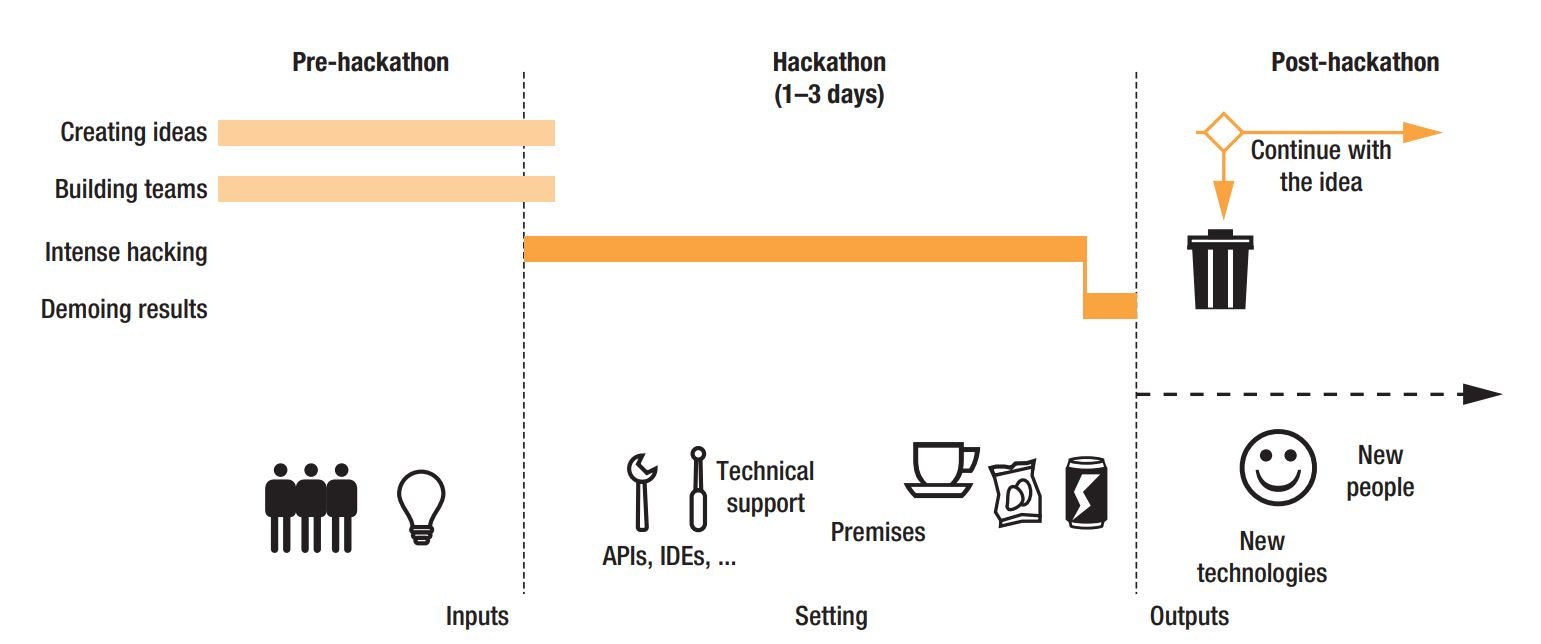
\includegraphics[width=0.75\linewidth]{hackprocess.JPG}
  \caption{Hackathon process adapted from \cite{komssi2014hackathons}} \label{Fig:hackprocess} 
 % \vspace{-20pt}
\end{figure*}
\end{comment}